% !TeX program = xelatex 

\PassOptionsToPackage{prologue, dvipsnames}{xcolor}
\documentclass[12pt]{exam}
\usepackage{lipsum}
\usepackage{graphicx}
\usepackage{listings}
\usepackage{xcolor}

% 支持中文的设置
\usepackage{xeCJK}
\usepackage{fontspec}
\setCJKmainfont[ItalicFont=思源宋体,BoldFont=SourceHanSerifSC-Bold]{Source Han Serif SC}
\newcommand{\KaiTi}{\CJKfontspec{楷体}}%用命令\fzkaiti调用方正楷体简体

\lstnewenvironment{cppcode}[1][]%
{
	\lstset{
		tabsize=4,
		language={C++},
		escapeinside=``,
		breaklines=true,
		breakatwhitespace=true, % 在空格处断行
		basicstyle=\ttfamily,
		keywordstyle=\color{blue}\ttfamily,
		stringstyle=\color{red}\ttfamily,
		commentstyle=\color{green}\ttfamily,
		morecomment=[l][\color{magenta}]{\#},
		literate={\ \ }{{\ \ \ \ }}4,
		#1
	}
}%
{}

\begin{document}
	\large
	\linespread{1.6} \selectfont
	
	\begin{center}
		\textbf{\large 技术面试题}
	\end{center}
	
	\begin{questions}
		
		\question
		\textbf{选择题:}
		\begin{figure}[htbp]
			\centering
			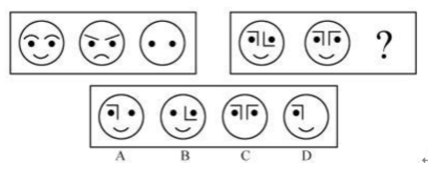
\includegraphics[width=\linewidth]{XOR}
			\caption{选择匹配?处的答案}
		\end{figure}
		
		\question
		\textbf{谈谈对下面代码的看法:}
		\begin{cppcode}
int* p;
*p = 100;
printf("*p=%d\n", *p);
		\end{cppcode}
	\end{questions}
	
\end{document}